% This is samplepaper.tex, a sample chapter demonstrating the
% LLNCS macro package for Springer Computer Science proceedings;
% Version 2.21 of 2022/01/12
%
\documentclass[runningheads]{llncs}
%
\usepackage[T1]{fontenc}
\usepackage{float}

% T1 fonts will be used to generate the final print and online PDFs,
% so please use T1 fonts in your manuscript whenever possible.
% Other font encondings may result in incorrect characters.
%
\usepackage{graphicx}
\usepackage{cite}
\usepackage{multirow}  % Required for \multirow command
\usepackage{subcaption}




% Used for displaying a sample figure. If possible, figure files should
% be included in EPS format.
%
% If you use the hyperref package, please uncomment the following two lines
% to display URLs in blue roman font according to Springer's eBook style:
%\usepackage{color}
%\renewcommand\UrlFont{\color{blue}\rmfamily}
%\urlstyle{rm}
%
\begin{document}
%
\title{Evaluating Deep Learning Methods for Detecting AI Generated Images: A Study on GenImage}
%
%\titlerunning{Abbreviated paper title}
% If the paper title is too long for the running head, you can set
% an abbreviated paper title here
%
\author{Isabela Iacob \and Emilia-Maria Nuță}
%
% First names are abbreviated in the running head.
% If there are more than two authors, 'et al.' is used.
%
\institute{Babeș-Bolyai University, Cluj-Napoca, România}
%
\titlerunning{DL Methods for Detecting AI Generated Images}
\maketitle              % typeset the header of the contribution
%
\begin{abstract}

In a world full of images and data, where artificial intelligence is now more powerful than ever and can generate complex and lifelike digital media, it is essential to maintain a well-defined line between real content and AI-generated creations. We can fight the misinformation where images generated by AI are used in malicious ways by training different AI models to identify and classify the real and the generated images. For this experiment, we use different machine learning models to classify the fake and real images: a custom CNN, a ResNet50, and a ConvNeXtSmall architectures.
The custom CNN architecture relies on multiple convolutional layers to extract hierarchical features from the images, pooling layers for dimensionality reduction, and fully connected layers for final classification. On the other hand, the ResNet introduces residual connections, or skip connections, allowing the network to mitigate the vanishing gradient problem and train deeper architectures effectively. ResNet is particularly well-suited for capturing complex patterns in image data by preserving information across layers.
We utilize the GenImage dataset, a large dataset containing both AI-generated images and real photographs, labeled as 'ai' or 'nature'.  We will present the final results of both architectures alongside the methodology and experiments conducted. Our findings show that the ConvNeXtSmall model outperforms the other two models, achieving an accuracy of 99\%.
These experiments are crucial in an era dominated by artificial intelligence to maintain ethical and secure use of media across the internet and to address potential future legal implications.

\keywords{Computer Vision  \and Deep Learning \and Generative AI}
\end{abstract}
%
% ---- Introduction ----
%
\section{Introduction}

Recently, the field of synthetic image generation through artificial intelligence (AI) has evolved rapidly, creating a critical need to detect these images to ensure authenticity and veracity. As AI-generated content becomes more sophisticated, detecting synthetic images will become increasingly challenging, posing significant risks in fields such as law, where the authenticity of visual evidence could influence the outcome of a case. This issue is particularly crucial when determining the veracity of images used in legal proceedings, where misidentification of AI-generated content could have serious consequences for justice.

Therefore, our research proposes the application and optimization of well-established deep learning architectures to detect AI-generated images. Additionally, we employ adversarial attacks on these architectures to assess their robustness and effectiveness in real-world scenarios, where attempts to deceive detection systems are becoming more prevalent. 

We also take into consideration the fast development that the Transformers architecture brought into the machine-learning world, by leveraging the architectures inspired by the transformer's architecture and design, such as networks from the ConvNext family, that are now widely used in machine-learning tasks, especially classification. 

The paper is structured into five main sections (excluding the introduction). Section 2 reviews the related work on detecting AI-generated images, as this area has become essential for ongoing research and development. We'll provide related work for the pre-trained architectures that we used, ResNet and ConvNeXt families. Even though they serve the same purpose and can be used in the completion of the same task, they are fundamentally different, which we will discuss in the Methodology section. Section 3 talks about the dataset used in the study: the GenImage dataset, a widely recognized collection of both AI-generated and real images. There are images from multiple sources and contain generated images and nature pictures.  Section 4 outlines the methodology used in our experiments, detailing the deep learning models applied and the approach for testing their robustness through adversarial attacks. In Section 5, we present the results obtained from our experiments, followed by an in-depth discussion of their implications. Finally, Section 6 concludes the paper, summarizing the key findings and suggesting potential future research directions in this rapidly advancing field.

The goal of our study is to compare how well each model performs in classifying images. We'll use standard metrics to measure their performance, such as accuracy, precision, and F1-score, to compare the results of the three techniques. 
%
% ---- Related work ----
%
\section{Related work}

\subsubsection{Existing detection techniques.} The accurate detection of AI-generated images is paramount, and as such there exist several deep learning approaches for this task. More prevalent are learning-based methods. Wang et al.~\cite{wang2019cnngenerated} use a ResNet-50 architecture pre-trained with the ImageNet as a classifier and train it in a binary classification setting using a ProGAN-generated dataset. They find that the CNN model could generalize well in the detection of other GAN-generated images. While research suggests that learning-based methods are viable for this task, Ojha et al.~\cite{ojha2023towards} show that real-vs-fake image classification models trained on a specific generative model have limited generalizability to other generative models and that the learned features are biased towards recognizing patterns from one class disproportionately better than the other. Other works~\cite{francesco2019fingerprint, ning2019fingerprint} present that AI-generated images have unique traces (called fingerprints) that depend on the architecture and training characteristics. Our work tries to train neural networks on data generated by different generative models and assess their performance.

\subsubsection{AI generated images.} The field of AI-generated images has rapidly evolved in the last years, mainly with the use of GANs (Generative Adversarial Networks) and DMs (Diffusion Models). In this study, we focus on this type of AI-generated images to determine whether different learning-based methods categorize them as fake or not, by combining and comparing classical ML techniques to more recent ones. Although the mentioned approaches are still used and provide very good results, thanks to the transformers architecture we are now able to have models that reach capabilities that were not seen before. For example, the DALL-E 2 model provided by OpenAI is a transformer-based model that combines transformer architectures with diffusion models. It uses a combination of two techniques: CLIP (Contrasive Language-Image Pre-training), which connects text and images by understanding the semantic relationship between them, and diffusion models. As AI-generated images(AIGI) are able to generate harmful, architectures such as CLIP are now more important than ever. CLIP is pre-trained on the datasets available on the internet, so it can differentiate the images generated by the different models available. The models learn to apply and maximize cosine similarity between the text embeddings and the images, and select the image with the highest cosine similarity. Therefore, the model is perfect for detecting the generated images, as it is able to adapt to the input domains, very important in AIGI detection models, as we want them to identify patterns and adapt to different images and domains\cite{moskowitz2024clip}. DALL-E 2 uses random noise in the beginning, and it continues to refine the image until it produces a high-quality image, guided by a text prompt ~\cite{ramesh2022clip}. It's important to mention that even though transformers played a huge role in the development of today's AI application, other approaches involve the use of more classic techniques, that are still very important and used. For example, the autoregressive models generate images pixel-by-pixel in a sequential manner, and one pixel depends on the previously generated one. It can generate very qualitative images for small datasets, by capturing strong dependencies between the pixel. One of these models, for example, is PixelCNN which uses convolutional layers for different applications, such as generating new portraits of the same person with different facial expressions or lighting conditions\cite{oord2016pixelcnn}.


%
% ---- Dataset ----
%
\section{Dataset}

In this study, we use the GenImage dataset~\cite{zhu2023genimage}, a comprehensive resource comprising over 2.6 million images, including 1.35 million AI-generated and 1.33 million real images. The dataset leverages 1,000 distinct labels from the ImageNet database, ensuring a diverse range of image categories that span various subjects such as animals, objects, and scenes. The image generation process for the GenImage dataset employs several state-of-the-art generative models. These include diffusion models such as Midjourney~\cite{midjourney}, Stable Diffusion V1.4~\cite{robin2022sd} and V1.5~\cite{robin2022sd}, GLIDE~\cite{nichol2022glide}, VQDM~\cite{shuyang2022vqdm} and ADM~\cite{dhariwal2021adm}, as well as GANs like BigGAN~\cite{brock2019largescalegantraining}. Since the original dataset proposed by the authors is very big in size, we use a tinier version of it available on Kaggle\footnote{https://www.kaggle.com/datasets/yangsangtai/tiny-genimage}. In the Kaggle version, just 5000 images are kept for 7 of the aforementioned generative models (Stable Diffusion V1.4 is excluded). For each model, data is divided into train (4000 images) and validation (1000 images), divided further into ai (2000 images for train and 500 images for validation) and nature (2000 images for train and 500 images for validation). GenImage uses the ImageNet dataset for the real images, and has images for each of the 1000 distinct labels. A sample of the dataset can be seen in Figure~\ref{fig:dataset-sample}.

\begin{figure}[ht]
    \centering
    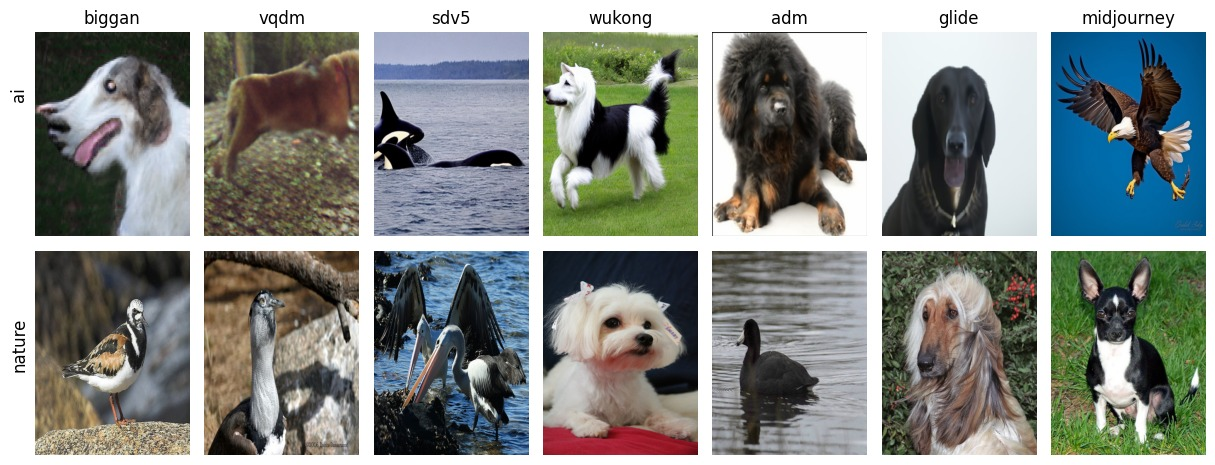
\includegraphics[width=0.8\textwidth]{graphics/dataset_sample.jpeg}
    \caption{Sample images from the GenImage dataset}
    \label{fig:dataset-sample}
\end{figure}

%
% ---- Methodology ----
%
\section{Methodology}

In this paper, we will address the task of classifying images into two categories: images that an AI model and real images generated. For this experiment, we employed a comprehensive approach that involves three different models: a model that uses a custom Convolutional Neural Network (CNN), a pre-trained ResNet model, and a ConvNextSmall network. In this section, we will provide details about the dataset preparation, the network architectures we used, and the evaluation metrics that we used to measure the performance of the three models. 

\subsubsection{Data preparation} 
As mentioned in a previous section, we used the GenImage dataset that contains several state-of-the-art generative models. The images were separated into different folders, with a training and a validation subfolder, both having two categories: ai and nature. We used all the training and validation images from all the folders, for better training. We further divided the validation images in half to create a test dataset. With this division, we were left with 4000 images for training, 500 for evaluation and 500 for testing. When creating the dataset structures used in the models, we resized them to a resolution of 224x224 for the ResNet50 and ConvNeXtSmall models, and 32x32 for our custom. The images were pre-processed to maintain compatibility with the models, especially with the pre-trained networks, and to standardize input dimensions across the models.

\vspace*{-2ex} % Force negative space
\begin{figure}[H]
    \centering
    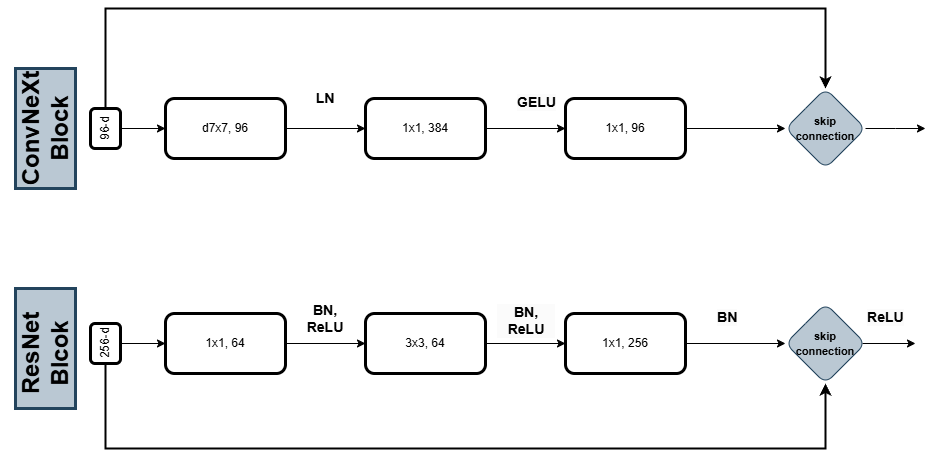
\includegraphics[width=\textwidth]{graphics/ConvRes.png} % Scale to fit the page width
    \caption{Differences between ConvNeXt and ResNet Architectures}
    \label{fig:custom-cnn}
\end{figure}
\vspace*{-2ex} % Force negative space
\subsubsection{Model Architectures}
\vspace*{-30ex} % Force negative space
As mentioned, for this task, we employed three model architectures:  a custom CNN designed specifically for the classification task, a ResNet model fine-tuned from pre-trained weights, and a ConvNextSmall network adapted for binary classification. 
The custom CNN used in this task was designed as a lightweight model that is suitable for image classification tasks. We implemented this architecture using TensorFlow and Keras, which consists of convolutional, pooling, and dense layers organized to facilitate effective classification. The model uses images of dimensions 32x32x3, and the process begins with three convolutional layers. We use the Rectified Linear Unit (ReLU) activation, padding "same", which ensures the output dimensions remain consistent with the input, and max-pooling operation, which reduces the spatial dimensions by half, to retain the most salient features. After the convolutional and pooling operations, the output feature maps are flattened into a one-dimensional vector with the use of a GlobalAveragePooling2D layer to prepare them for the dense layers, which consist of 128 neurons with ReLU activation and a dropout layer with a rate of 0.5, to mitigate overfitting by randomly deactivating half of the neurons during training. The output layer is a dense layer with just one neuron, and it utilizes a sigmoid activation function. These techniques provide class probabilities for the binary classification task. The model is compiled using the gradient descent (SGD) optimizer, and the binary cross-entropy loss function is used. The whole architecture can be seen in Figure~\ref{fig:custom-cnn}.


\begin{figure}[H]
    \centering
    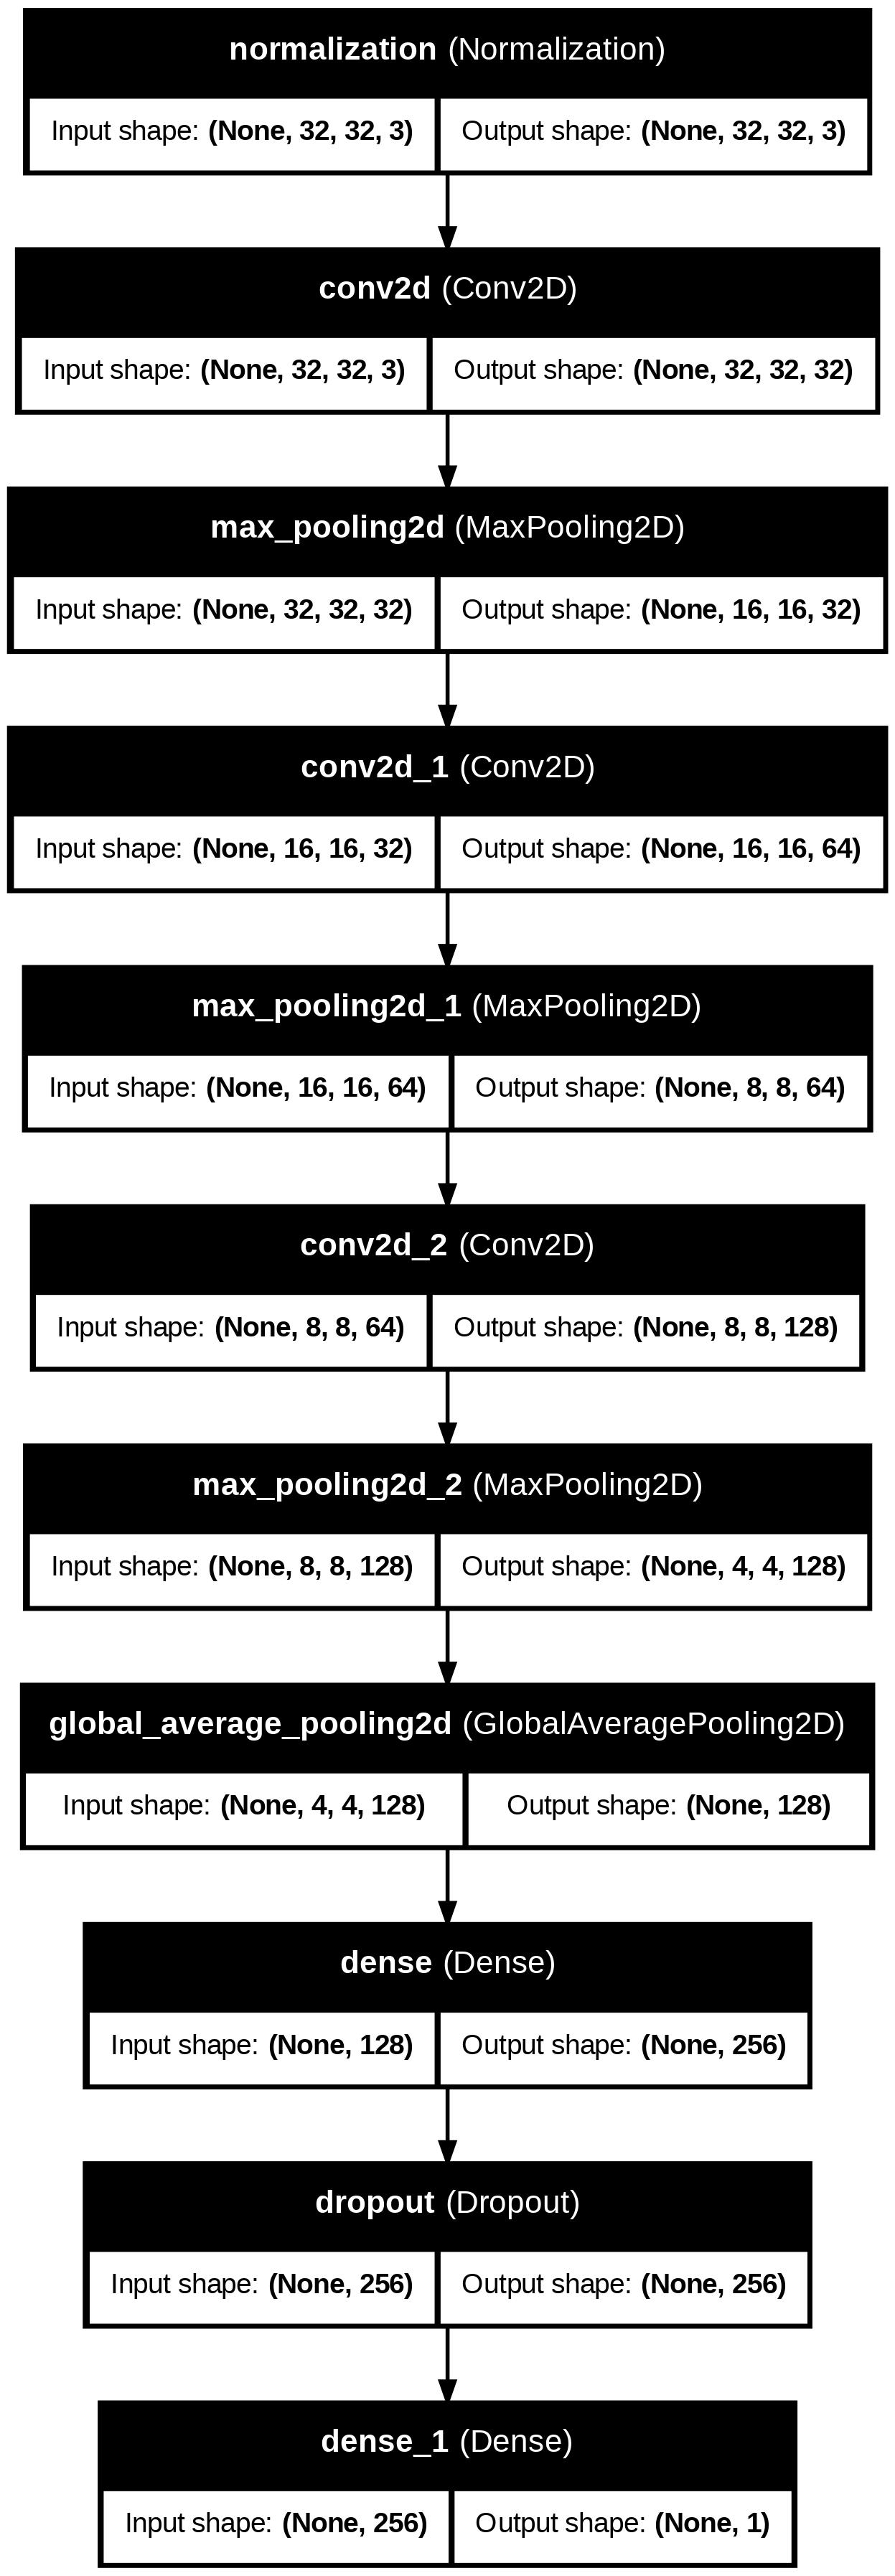
\includegraphics[height=13cm]{graphics/custom_model.png}
    \caption{Structure of custom model}
    \label{fig:custom-cnn}
\end{figure}

Resnet50 is a deep CNN architecture that introduced residual learning, a concept that was proposed to solve the vanishing gradient problem in very deep networks. It was developed as part of the ResNet family, and this specific version (ResNet50) became popular and a widely used architecture, especially in image classification. When it comes to fundamental elements, this architecture uses residual blocks, which introduce a shortcut connection, allowing the network to learn residual mappings instead of deep mappings. ResNet50 consists of 50 layers, 48 convolutional layers, 1 max-pooling, and 1 average pooling layer. Another important aspect of this architecture is its parameter number, approximately 25.6 million, a modest number compared to other architectures from the ResNet family. Moreover, using bottleneck blocks makes ResNet50 efficient without losing accuracy points. For our experiment, the model was initialized with ImageNet weights to capitalize on pre-learned features, this dataset having over a million images across 1000 categories. This way, our model has a strong baseline of generalized features instead of learning from scratch, like in the first example. The top classification layer of ResNet50 was removed so we can better adapt the network for our task to append custom layers for our classification task. Now, the model accepts inputs of 224x224x3, consistent with the ResNet50 architecture. We wanted to ensure that the model's baseline remained intact, meaning that we wanted the model to keep the generic features. Therefore, we froze the convolutional layers of the base model. This way, the base layers will not be updated during training, saving a lot of computational costs and risk regarding overfitting. A custom classification head is appended to the base model to fine-tune the base model for our task, a binary classification consisting of several elements: global average pooling, a fully connected layer, which is essentially a dense layer with 256 neurons, and ReLU activation, a dropout layer, with the same scope as the one used in the first experiment with the custom network, where we deactivated half of the neurons and an output layer, a dense layer with a single neuron and sigmoid activation, where the output values closer to 0 indicate AI-generated images, and values closer to 1, real photos. The model was compiled using binary cross-entropy as a loss function; as an optimizer, we used SGD, and as a default metric, we selected accuracy. 

ConvNext is a modern architecture inspired by the design of transformer-based vision models~\cite{liu2022convnet}. To summarize, ConvNext tries to combine CNN's performance with the improvements brought by transformers. ConvNextSmall is a lighter version of the ConvNext family that adopts design choices from the Swin Transformer~\cite{liu2021swin}, a multi-scale transformer architecture that is well-designed for high-resolution images in computer vision. The implementation of the two architectures, using the Keras API and the processes that allow us to use the pre-trained network for a specific classification task,  is quite similar, but the two architectures are fundamentally different. We used the Gaussian Error Linear Unit (GeLU) activation function, which is very commonly used in Transformers. GeLU function weights inputs by their value and uses a probabilistic approach, using the Gaussian cumulative distribution function. In contrast, the ReLU function outputs the input directly if it is positive and 0 if it is not. While ReLU is much easier to compute, GeLU works perfectly in reducing the changes in gradients, making the optimization more stable. Another important aspect is related to the building of blocks. If ReSnet50 used Residual BottleNeck Blocks, for ConvNextSmall, we have Simplified ConvNext Blocks, modern blocks that use both CNN and transformer design principles.

%
% ---- Results and discussion ----
%
\section{Results and discussion}
All the aforementioned experiments were run on Google Colab resources using the A100 GPU runtime. The training process was done for 50 epochs, with a batch size of 32. Due to the costs involved, we tried to minimize the time spent on training and utilized EarlyStopping from the Keras API to halt the training process when the validation loss did not decrease for 5 epochs. We also used ReduceLROnPlateau in order to reduce the learning rate by a factor of 0.1 when the validation loss did not decrease for 2 epochs. For experimentation consistency, we used the random seed set to 0. The results of the three models are presented in Table~\ref{tab:simpleresults}.

\begin{table}
    \centering
    \caption{Results of the three models on the GenImage dataset.}\label{tab1}
    \begin{tabular}{l|c}
    \hline
    Method & Accuracy (\%) \\
    \hline
    Custom &  74.4 \\
    ResNet50 & 98.2 \\
    ConvNeXtSmall & 99 \\
    \hline
    \end{tabular}
    \label{tab:simpleresults}
\end{table}

As can be seen from the results, the ConvNeXtSmall model outperforms the other two models, achieving an accuracy of 99\%. The ResNet50 model also performs well, with an accuracy of 98.2\%, while the custom CNN model has an accuracy of 74.9\%. The results show that the ConvNeXtSmall model is the most effective at classifying AI-generated images, while the ResNet50 model is also highly accurate. The custom CNN model, however, is less effective at classifying AI-generated images, suggesting that more complex models may be better suited to this task. The smaller image size used in the custom CNN model may also have contributed to its lower accuracy, as it may not have been able to capture the necessary details to classify the images accurately. Overall, the results suggest that more complex models, such as the ConvNeXtSmall and ResNet50 models, are better suited to the task of classifying AI-generated images, while simpler models may struggle to classify these images accurately. By comparison, similar results were obtained for the ResNet50 architecture, where the GenImage authors obtained an accuracy of 99.5\%  on the entire dataset~\cite{zhu2023genimagesupp}. The plots of the accuracy and loss for the three models can be seen in Figure~\ref{fig:sixgraphs}.

\begin{figure}[htbp]
    \centering
    \begin{subfigure}[b]{0.45\textwidth}
        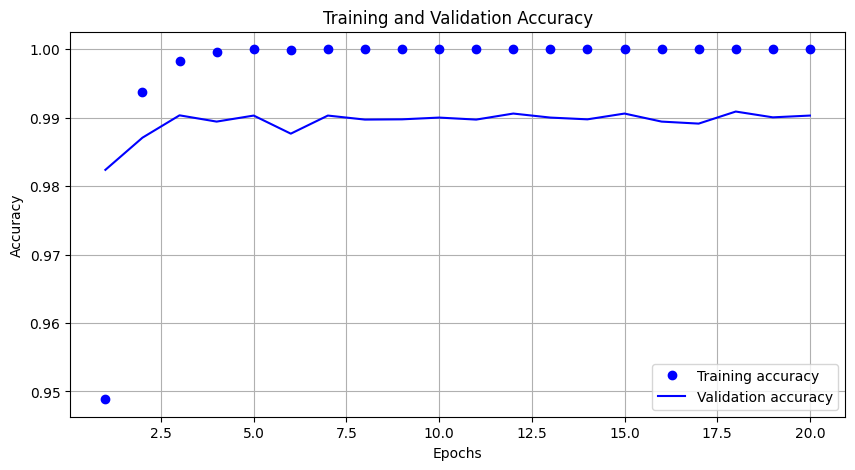
\includegraphics[width=\textwidth]{graphics/accuracy_resnet.png}
        \caption{ResNet50 accuracy}
        \label{fig:graph1}
    \end{subfigure}
    \hfill
    \begin{subfigure}[b]{0.45\textwidth}
        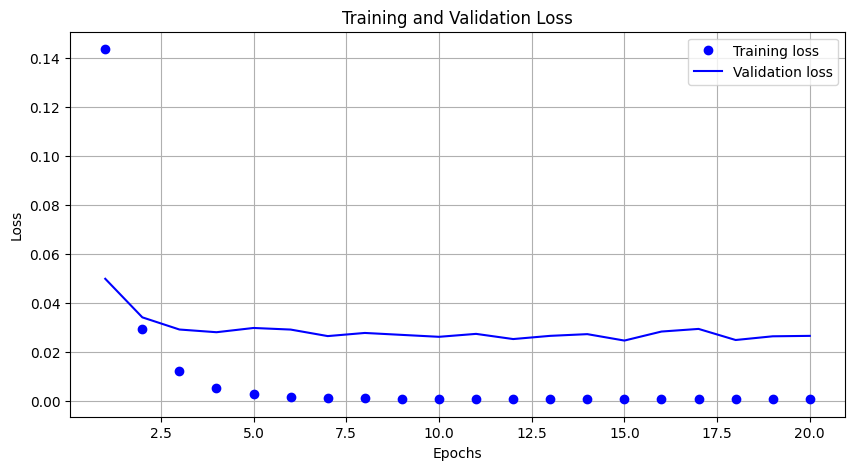
\includegraphics[width=\textwidth]{graphics/loss_resnet.png}
        \caption{ResNet50 loss}
        \label{fig:graph2}
    \end{subfigure}

    \vspace{0.5cm}

    \begin{subfigure}[b]{0.45\textwidth}
        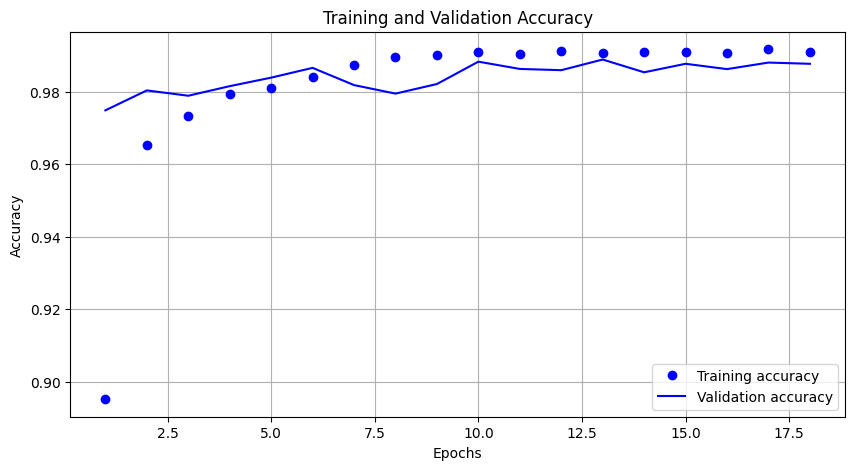
\includegraphics[width=\textwidth]{graphics/accuracy_convnext.png}
        \caption{ConvNeXtSmall accuracy}
        \label{fig:graph3}
    \end{subfigure}
    \hfill
    \begin{subfigure}[b]{0.45\textwidth}
        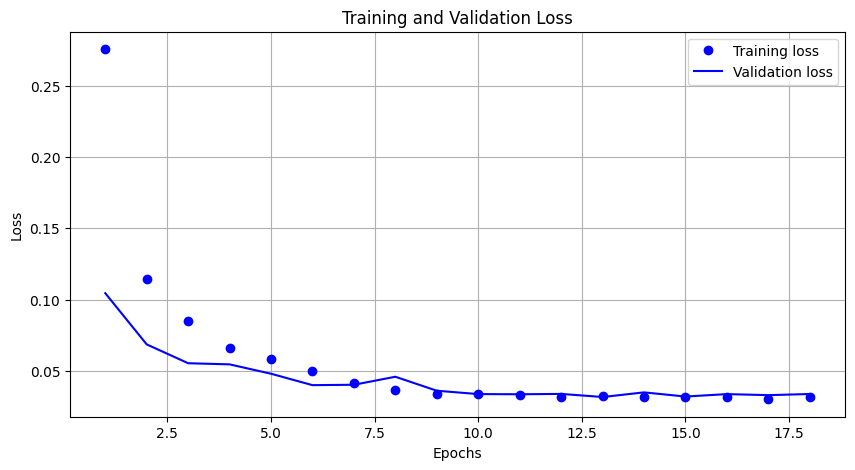
\includegraphics[width=\textwidth]{graphics/loss_convnext.png}
        \caption{ConvNeXtSmall loss}
        \label{fig:graph4}
    \end{subfigure}

    \vspace{0.5cm}

    \begin{subfigure}[b]{0.45\textwidth}
        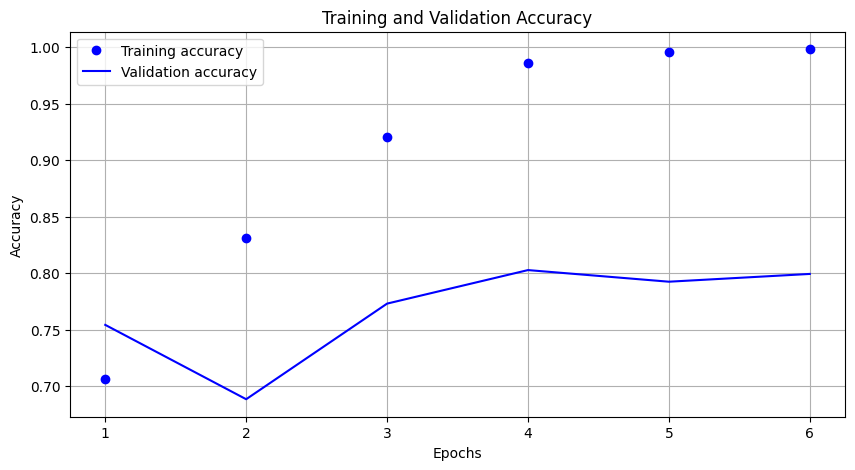
\includegraphics[width=\textwidth]{graphics/accuracy_custom.png}
        \caption{Custom model accuracy}
        \label{fig:graph5}
    \end{subfigure}
    \hfill
    \begin{subfigure}[b]{0.45\textwidth}
        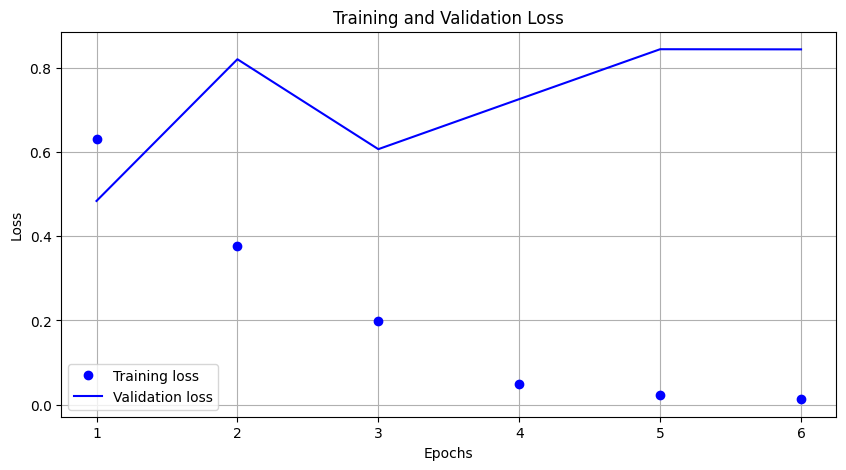
\includegraphics[width=\textwidth]{graphics/loss_custom.png}
        \caption{Custom model loss}
        \label{fig:graph6}
    \end{subfigure}

    \caption{Accuracy and loss plots for the ResNet50, ConvNeXtSmall and custom models.}
    \label{fig:sixgraphs}
\end{figure}


Following the works of~\cite{wang2019cnngenerated}, since detectors are supposed to be robust, we tested these models on an augmented test dataset to simulate real world degradation of the images (e.g. compression, noise interference and low resolution). For these experiments, we augmented the test dataset into 4 variants: gaussian blur with the standard deviation of the Gaussian distribution sampled randomly within the range [0,3], jpeg compression with a quality level randomly within the range [30, 100], and blur+jpeg with each a 50\%, respectively a 10\% probability of happening.

\begin{table}[h]
    \centering
    \caption{Results on augmented test dataset.}
    \begin{tabular}{c|c|c|c|c|c}
    \hline
    \multirow{2}{*}{Method} & \multicolumn{4}{c|}{Testing subset} & \multirow{2}{*}{Avg acc (\%)} \\ \cline{2-5}
                                      & Blur & JPEG & Blur+JPEG (p=0.5) & Blur+JPEG(p=0.1) & \\ \hline
    Custom                            & 63.7   & 64.5   & 59.1   & 75.1   & 50.8 \\ \hline
    ResNet50                          & 80.1   & 68.9   & 64.1   & 84.5   & 74.4 \\ \hline
    ConvNeXtSmall                     & 82.4   & 72.9   & 66.0   & 93.9   & 78.8 \\ \hline
    \end{tabular}
    \label{tab:augmentedresults}
\end{table}

As can be seen from the results in Table~\ref{tab:augmentedresults}, the ConvNeXtSmall model again outperforms the other two models, achieving an average accuracy of 78.8\%. The ResNet50 model also performs well, with an average accuracy of 74.4\%, while the custom CNN model has an average accuracy of 50.8\%. The results show that the ConvNeXtSmall model is the most robust to image degradation, while the ResNet50 model is also highly robust. The custom CNN model, however, is less robust to image degradation, suggesting that more complex models may be better suited to this task. The smaller image size used in the custom CNN model may also have contributed to its lower robustness, as it may not have been able to capture the necessary details to accurately classify the images.
%
% ---- Conclusion ----
%
\section{Conclusion}

To conclude, our study demonstrates the effectiveness of deep learning models in classifying AI-generated images. We compared the performance of three models: a custom CNN, a ResNet50, and a ConvNeXtSmall architecture, on the GenImage dataset. As expected, our results show that the ConvNeXtSmall model outperforms the other two models, achieving an accuracy of 99\%. Thanks to the improvements brought by transformers, combined with the CNN's performance we were able to achieve impressive results, with an error rate of only 1\%.  We also tested the models on an augmented test dataset to simulate real-world degradation of the images, and found that the ConvNeXtSmall model is the most robust to image degradation, achieving an average accuracy of 78.8\%. Our findings suggest that more complex models, such as the ConvNeXtSmall and ResNet50 models, are better suited to the task of classifying AI-generated images, while simpler models may struggle to accurately classify these images, without using complex architectures. Future work could involve further testing the models on a larger dataset, as well as exploring other deep learning architectures to improve the classification of AI-generated images. There is also the question of whether these models could perform well on other datasets, generated by different generative models that were not used in the training phase, especially  models that are now able to generate more accurate images, such as DALL-E 3, MidJourney v5, recent versions of Stable Diffusion and other advanced models. 
%
% ---- Bibliography ----
%
% BibTeX users should specify bibliography style 'splncs04'.
% References will then be sorted and formatted in the correct style.
%
\bibliographystyle{splncs04}
\bibliography{references}

\end{document}
